\onecolumn
\chapter{Auswertung}
% Liste der genutzer Formeln für die Fehlerrechnung
\section*{Fehlerrechnung}
Für die statistische Auswertung von $n$ Messwerten $x_i$ werden folgende Größen definiert \cite{errorSkript25}:
\begin{align}
    \bar{x} &= \frac{1}{n} \sum_{i=1}^{n} x_i \vphantom{\sqrt{\sum_i^n}^2} && \text{\textcolor{gray}{Arithmetisches Mittel}} \label{eq:arithmetisches_mittel} \\
    \sigma^2 &= \frac{1}{n-1} \sum_{i=1}^{n} (x_i - \bar{x})^2 \vphantom{\sqrt{\sum_i^n}^2} && \text{\textcolor{gray}{Variation}} \label{eq:variation} \\
    \sigma &= \sqrt{\frac{1}{n-1} \sum_{i=1}^{n} (x_i - \bar{x})^2} \vphantom{\sqrt{\sum_i^n}^2} && \text{\textcolor{gray}{Standardabweichung}} \label{eq:standardabweichung} \\
    \Delta \bar{x} &= \frac{\sigma}{\sqrt{n}} = \sqrt{\frac{1}{n(n-1)} \sum_{i=1}^n(\bar x - x_i)^2} \vphantom{\sqrt{\sum_i^n}^2} && \text{\textcolor{gray}{Fehler des Mittelwerts}} \label{eq:fehler_mittelwert} \\
    \Delta f &= \sqrt{\left(\frac{\partial f}{\partial x} \Delta x\right)^2 + \left(\frac{\partial f}{\partial y} \Delta y\right)^2} \vphantom{\sqrt{\sum_i^n}^2} && \text{\textcolor{gray}{Gauß’sches Fehlerfortpflanzungsgesetz für $f(x,y)$}} \label{eq:gauss_fehlfortpflanzung} \\
    \Delta f &= \sqrt{(\Delta x)^2 + (\Delta y)^2} \vphantom{\sqrt{\sum_i^n}^2} && \text{\textcolor{gray}{Fehler für $f = x + y$}} \label{eq:fehler_summe} \\
    \Delta f &= |a| \Delta x \vphantom{\sqrt{\sum_i^n}^2} && \text{\textcolor{gray}{Fehler für $f = ax$}} \label{eq:fehler_proportional} \\
    \frac{\Delta f}{|f|} &= \sqrt{\left(\frac{\Delta x}{x}\right)^2 + \left(\frac{\Delta y}{y}\right)^2} \vphantom{\sqrt{\sum_i^n}^2} && \text{\textcolor{gray}{relativer Fehler für $f = xy$ oder $f = x/y$}} \label{eq:relativer_fehler} \\
    \sigma &= \frac{|a_{lit} - a_{gem}|}{\sqrt{\Delta a_{lit}^2 + \Delta a_{gem}^2}} \vphantom{\sqrt{\sum_i^n}^2} && \text{\textcolor{gray}{Berechnung der signifikanten Abweichung}} \label{eq:signifikante_abweichung}
\end{align}

\twocolumn

\section{Graphische Bestimmung des Richtmomentes}
Kommen wir also nun zur Auswertung der Aufgaben. Dafür Beginnen wir damit, die Werte der Tabelle 1  aus dem \hyperref[Protokoll]{Protokoll}.
Dabei ist $x$ die Winkelauslenkung der Aluminiumscheibe, $m$ hängende Masse, $F$ die Gewichtskraft mit $\left| g \right| =9,81 \frac{m}{s^2}$, die auf die Masse wirkt $M$ das berechnete Drehmoment nach \hyperref[eq:gleichgewichts_zustand]{Gleichung 2.1} und $\Delta M$ seine Ungenauigkeit nach der \hyperref[eq:gauss_fehlfortpflanzung]{Gauß'schen Fehlerfortpflanzung}:
\begin{equation}
    \Delta M = \left| m \right| \cdot \left| g \right| \cdot \Delta r
\end{equation}
Dabei definieren die 0g den Startpunkt. 0g ist physikalisch in dem Kontest natürlich unsinnig und meint eigentlich die Startmasse, die hier nur aus dem Massenteller besteht, aber keine zusätzliche Masse.
Der Radius der Aliminumplatte entspricht dabei $r = 10,000 \pm 0,005 \, 10^{-2}m$, also ist $\Delta r = 0,005 \, 10^{-2}m$, was der Ungenauigkeit der Schieblehre entspricht.
\begin{table}[h!]
    \begin{tabular}{c | c | c | c }
    $m [g]$ & $\varphi [^{\circ}]$ & $M \, [10^{-2}Nm]$ & $\Delta M \, [10^{-2}Nm]$ \\
    \hline
    0   & 0   & ---     &  ---    \\
    50  & 60  &  4,9050 & 0,0024525 \\
    100 & 122 &  9,8100 & 0,0049050 \\
    150 & 180 & 14,4150 & 0,0073575 \\
    200 & 242 & 19,6200 & 0,0098100 \\
    250 & 302 & 24,5250 & 0,0012263 \\
    300 & 366 & 29,4300 & 0,0014715 \\
    \hline
    \end{tabular}
    \caption{Messungen der Rotationsauslenkung der Aluminumscheibe und die berechneten Drehmomente.}
    \label{tab:verschiedene_massen_winkel_auslenkung}
\end{table}

Stellen wir nun \hyperref[eq:kraft_drehmoment_zusammenhang]{Gleichung 1.3} um, so kommen wir auf:
\begin{equation}
    D_G = - \frac{M}{\varphi}
\end{equation}

Daher plotten wir als nächstes das Drehmoment $M$ gegen den Auslenkungswinkel $\varphi$ und berechnen seine Steigung $m$, welche dem Drehmoment entspricht, nach
\begin{equation}
    m = \frac{\Delta M}{\Delta \varphi}
\end{equation}

Dies kann der \hyperref[img:graphisch_richtmoment]{Abbildung zur Bestimmung des Richtmomentes} entnommen werden. Dabei rechnen wir Gradmaß in Radiant um. Es gilt:
\begin{equation}
    x^\circ \cdot \frac{\pi}{180} = y \, rad
\end{equation}  
Somit kommen wir auf Steigungen von:
\begin{align}
    m_A &= \frac{0,230 Nm}{5,4105 rad} = 0,043 \, \frac{Nm}{rad} = D_{G,A}\\
    \nonumber \\ 
    m_F &= \frac{0,259 Nm}{5,4105 rad} = 0,048 \, \frac{Nm}{rad}
\end{align}

Dabei ist $m_A$ die Steigung der Ausgleichsgeraden und $m_F$ die Steigung der Fehlergeraden, welche über das Min.-Max.-Verfahren bestimmt wurde. $\Delta \varphi$ sind dabei $2^\circ$.

Zieht man nun deren Differenz, so kommt man auf einen Fehler variation
\begin{align}
    \Delta D_G &= \left| m_F - m_A \right| \\ 
            &= \left| 0,048 - 0,043 \right| = \underline{0,005} \, \Big[\frac{Nm}{rad}\Big]
\end{align}
Damit können wir $D_G$ über $D_G = D_{G,A} \pm \Delta D_G$ bestimmen: 
\begin{equation}
    \underline{\underline{D_G = (4,3 \pm 0,5) \, 10^{-2}\frac{Nm}{rad}}}
    \label{e:d_g}
\end{equation}


\section{Rechnerische Bestimmung des Richtmomentrs}
\label{aufgabe_3-2}
Wir entnehmen die Werte aus dem \hyperref[Protokoll]{Protokoll} und schauen uns Tabelle 2 an. Wir haben die Schwingdauer $t$ für 20 Schwingungen, 
woraus sich auch die Periodendauer $T$ bestimmt. Der Durchschnitt der Periodendauer ohne Scheibe ist $\bar{T}_1$, und der mit der Scheibe $\bar{T}_2$.
Den Fehler der der Periodendauer $\Delta \bar{T}$ wurde über eine Reaktionszeit von $0,2s$ über \hyperref[eq:gauss_fehlfortpflanzung]{Gauß'sche Fehlfortpflanzung} berechnet sich der Fehler zu:
\begin{equation}
    \Delta \bar{T}_{reak} = 0,20\,\mathrm{s} \cdot \frac{1}{20} = 0,01\,\mathrm{s}
\end{equation}

Die Berechnung der \hyperref[eq:fehler_mittelwert]{Ungenauigkeit des Mittelwertes} wird zusätzlich vorgenommen:
\begin{align}
    \Delta \bar{T}_{1,stat} &= 0,003\,\mathrm{s} \\
    \Delta \bar{T}_{2,stat} &= 0,002\,\mathrm{s}.
\end{align}

Nun müssen beide Fehler über \hyperref[eq:gauss_fehlfortpflanzung]{Gauß'sche Fehlerfortpflanzung} zu einem zusammengeführt werden:
\begin{equation}
\Delta \bar{T}_{i} = \sqrt{(\Delta \bar{T}_{reak})^2 + (\Delta \bar{T}_{i,stat})^2}
\end{equation}

Wir kommen dabei auf Werte von:
\begin{align}
    \Delta \bar{T}_1 &= 0,010 \\
    \Delta \bar{T}_2 &= 0,010.
    \label{eq:t_reak}
\end{align}

Wir merken also: die Berechnete statistische Ungenauigkeit war hier nicht von Relevanz.

\begin{table}[h!]
    \begin{tabular}{c | c | c | c | c}
    Scheibe & $t \, [s]$& $T \, [s]$ & $\bar{T} \, [s]$ & $\Delta \bar{T} [s]$\\
    \hline
    Keine       & 23,09 & 1,155 & 1,162 & 0,010\\
                & 23,31 & 1,166 & $= \bar{T}_1$ & \\
                & 23,28 & 1,164 &  & \\
     \hline
    Messing-    & 34,89 & 1,745 & 1,741 & 0,010\\
    Platte      & 34,75 & 1,738 & $= \bar{T}_2$ & \\
                & 34,78 & 1,739 &  & \\
    \hline
    \end{tabular}
    \caption{Messungen der Schwingdauer einer regelmäßigen Messingplatte unter 20 Schwingungen.}
    \label{tab:regelmäßige_messingplatte}
\end{table}

Damit stehen unsere zwei Periodendauern fest, die wir für die Bestimmung des Richtmomentes $D_R$ brauchen:
\begin{align}
T_1 = (1,162 \pm 0,010)\,\mathrm{s} \\
T_2 = (1,741 \pm 0,010)\,\mathrm{s}.
\end{align}

Für die weitere Berechnung brauchen wir außerdem die Werte der Messingscheibe:
\begin{align*}
    \text{Durchmesser: }         d_M   &= 110\,\mathrm{mm}    &&\pm 0,005\,\mathrm{mm} \\
    \Rightarrow \text{Radius: }  r_M   &= 55\,\mathrm{mm}     &&\pm 0,0025\,\mathrm{mm} \\
    \text{Masse: }               m_M   &= 646\,\mathrm{g}     &&\pm 1\,\mathrm{g}
\end{align*}

Wir transferieren diese erstmal in typische SI-Einheiten:
\begin{align*}
    \text{Durchmesser: }         d_M   &= (0,110 \pm 0,000005)\,\mathrm{m} \\
    \Rightarrow \text{Radius: }  r_M   &= (0,055  \pm 0,0000025)\,\mathrm{m} \\
    \text{Masse: }               m_M   &= (0,646 \pm 0,001)\,\mathrm{kg}
\end{align*}

Damit greifen wir auf \hyperref[eq:richtmoment_rechnen]{Gleichung 1.9} zurück, um das Richtmoment zu bestimmen:
\begin{equation}
    D_R = \frac{2\pi^2 \cdot m_M \cdot r_M^2}{T_2^2-T_1^2}
\end{equation}

Nur noch bekannte Werte einsetzen:

\begin{align}
    D_R &= \frac{2\pi^2 \cdot 0,646\,\mathrm{kg} \cdot (0,055\,\mathrm{m})^2}{(1,741\,\mathrm{s})^2-(1,162\,\mathrm{s})^2} \\
    D_R &= \underline{0,022948 \,\mathrm{\frac{Nm}{rad}}}
    \label{eq:richtmoment_berechnet}
\end{align}

Somit brauchen wir für den Aufgabenteil nur noch den Fehler des Richtmomentes $\Delta D_R$. Wir greifen erneut auf die \hyperref[eq:gauss_fehlfortpflanzung]{Gauß'sche Fehlerfortpflanzung} zurück:

\begin{equation}
    \begin{split}
    \Delta D_R &= \Bigg[ 
    \left(\frac{\Delta m_M}{m_M}\right)^2 + 
    \left(\frac{\Delta r_M}{r_M}\right)^2 \\[6pt]
    &+ \left(\frac{2T_2 \Delta T_2}{T_2^2-T_1^2}\right)^2 
    + \left(\frac{2T_1 \Delta T_1}{T_2^2-T_1^2}\right)^2
    \Bigg]^{1/2} \cdot D_R
    \end{split}
\end{equation}

Setzen wir alle Werte ein, so kommen wir in unserem Fall auf eine Ungenauigkeit von:
\begin{equation}
    \underline{\Delta D_R = 0,00057265 \, \mathrm{\frac{Nm}{rad}}}
    \label{eq:richtmoment_fehler}
\end{equation}

Fassen wir \hyperref[eq:richtmoment_berechnet]{Gleichung 3.29} und \hyperref[eq:richtmoment_fehler]{Gleichung 3.31} zusammen und runden alles sinnvoll, so kommen wir auf:
\begin{equation}
    \underline{\underline{D_R = (2,29 \pm 0,06) \cdot 10^{-2}\,\mathrm{\frac{Nm}{rad}}}}
    \label{e:d_r}
\end{equation}


\section{Stein'scher Satz}
\label{aufgabe_3-3}
Die Aufgaben 3 bis 5 beschäftigen sich alle mit dem \hyperref[eq:steinsatz]{Stein'schen Satz}. 
Es wurde wieder die Schwingdauer $t$ für 20 Schwingungen gemessen. 

Zunächst nehmen wir die Gleichung zur \hyperref[eq:T_def]{Berechnung der Periodendauer (1.10)} und stellen diese nach $J_T$ um:
\begin{equation}
    J_T = \frac{T_1^2 \cdot D}{4\pi^2}
    \label{eq:j_t}
\end{equation}

Wir definieren die Periodendauer $T_P$ für die unregelmäßige Messingplatte, die das Trägheitsmoment $J_P$ hat. Diese benutzt die Formel zur \hyperref[eq:T_def]{Berechnung der Periodendauer (1.11)}:
\begin{equation}
    T_P = 2\pi \sqrt{\frac{J_T+J_P}{D}}.
\end{equation}

Nur noch nach $J_P$ umformen:
\begin{equation}
    J_P = \frac{T_P^2 \cdot D}{4\pi^2} - J_T.
\end{equation}

Nun setzen wir \hyperref[eq:j_t]{$J_T$} noch ein und erhalten:
\begin{equation}
    J_P = \frac{T_P^2 \cdot D}{4\pi^2} - \frac{T_1^2 \cdot D}{4\pi^2}.
\end{equation}

Nur noch vereinfachen:
\begin{equation}
    J_P = \frac{D}{4\pi^2}(T_P^2-T_1^2).
\end{equation}

Zudem wird die Ungenauigkeit nach \hyperref[eq:gauss_fehlfortpflanzung]{Gauß'schen Fehlerfortpflanzung} berechnet zu:
\begin{align}
\Delta J_P &= \Bigg[
    \left( \frac{T_P^2 - T_1^2}{4\pi^2} \, \Delta D \right)^2
    + \left( \frac{D T_P}{2\pi^2} \, \Delta T_P \right)^2 \notag \\[6pt]
&\quad
    + \left( \frac{D T_1}{2\pi^2} \, \Delta T_1 \right)^2
\Bigg]^{1/2} \cdot J_P
\end{align}

Dies sind die Formeln, die wir für die weitere Berechnung benötigen. Wir rechnen mit einer Periodendauer von $T_P = (2,221 \pm 0,010)\, \mathrm{s}$.
Genau so machen wir gebrauch von $T_1 = (1,162 \pm 0,010)\, \mathrm{s}$.

Wir werden zwei Rechnungen durchführen, einmal für $D_G =(4,3 \pm 0,5) 10^{-2} \mathrm{\frac{Nm}{rad}}$ und einmal für
$D_R =(2,29 \pm 0,06) 10^{-2} \mathrm{\frac{Nm}{rad}}$. Wir werden dann in der \hyperref[Diskussion]{Diskussion} die Graphische und die rechnerische Methode vergleichen.

Wir berechnen zunächst die Drehmomente und anschließend ihre Ungenauigkeiten:
\begin{equation}
    J_{P,G} = 3,9021744120 \, [\mathrm{10^{-3} kg \cdot m^2}]
    \label{eq:J_P_G}
\end{equation}

\begin{equation}
    J_{P,R} = 2,631699022 \, [\mathrm{10^{-3} kg \cdot m^2}]
    \label{eq:J_P_R}
\end{equation}

Nun müssen wir noch deren Ungenauigkeiten bestimmen:
\begin{equation}
    \Delta J_{P,G} = 0,017833522 \, [\mathrm{10^{-3} kg \cdot m^2}]
\end{equation}

\begin{equation}
    \Delta J_{P,R} = 0,0017299 \, [\mathrm{10^{-3} kg \cdot m^2}]
\end{equation}

Nun Fassen wir alle Ergebnisse sinnvoll zusammen und runden entsprechend: 
\begin{align}
    &\underline{\underline{J_{P,G} = (39,022 \pm 0,018)\, \mathrm{10^{-4}kg \, m^2}}} \\
        \notag \\
    &\underline{\underline{J_{P,R} = (26,3170 \pm 0,0017 )\, \mathrm{10^{-4} kg \, m^2}}}
    \label{e:s_t}
\end{align}

Nun haben wir für die Schwerpuntkachse $a_0$ das Trägheitsmoment bestimmt. Nun stellt sich noch die Frage nach den anderen Achsen. Erstmal suchen wir uns alle interessanten Größen wieder zusammen:
Dabei fassen wir die Tabellen 3 und 4 des \hyperref[Protokoll]{Protokolls} zusammen und berechnen die Periodendauer, das Trägheitsmoment $J_{a_i}$ analog zu \hyperref[aufgabe_3-3]{Aufgabe 3.3 (37)}, und darüber das Trägheitsmoment $J_{S_i}$ über den \hyperref[eq:steinsatz]{Stein'schen Satz (1.7)}.
Die Abstäne sind mit einem Millimetergeodreieck bestimmt wurden, dessen Ungenauigkeit lässt sich auf 
\begin{equation}
    \Delta d = 0,5mm = 50\% \cdot 1mm
\end{equation}
abschätzen. Für die Ungenauigkeit der $\Delta T$ berufen wir uns auf die Werte aus \hyperref[eq:t_reak]{Aufgabe 3.2 (23)}:
\begin{equation}
    \Delta T = 0,010 s.
\end{equation}
Zudem sind die Werte in der Tabelle bereits auf signifikante Stellen gerundet. 
Der Abstand $d$ wir im Stein'schen Satz quadrietr, somit müssen wir seinen Fehler via \hyperref[eq:gauss_fehlfortpflanzung]{Gleichung 3.7} berechnen:
\begin{equation}
    \Delta d^2 = 2d \Delta d.
\end{equation}

Die gesamte Ungenauigkeit wird sich nach \hyperref[eq:fehler_summe]{Gleichung 3.6} auf
\begin{equation}
    \Delta J_{S_i} = \sqrt{(\Delta J_{a_i})^2 + ({d_i}^2 \Delta m)^2 + (m \Delta {d_i}^2)^2}
\end{equation}
belaufen. Dabei nutzen wir $\Delta m = 1g$.

Zuletzt werden noch für jedes Trägheitsmomentes die \hyperref[eq:signifikante_abweichung]{$\sigma$-Abweichung} von $J_{a_i}$ zu den Trägheitsmomenten nach der Berechnung mit dem \hyperref[eq:steinsatz]{Stein'schen Satz (1.7)} $J_{S_i}$.

\begin{table}[h]
    \centering
    \begin{tabular}{c | c | c | c | c || c}
        Achse & $d^2 \,[10^{-4}\text{m}^2]$ & $T \,[\text{s}]$ & $J_{a_i}(D_G)\,[10^{-4}\text{kg}\cdot \text{m}^2]$ & $J_{S_i}(D_G)\,[10^{-4}\text{kg}\cdot \text{m}^2]$ & $\sigma_{a_G}$ \\
        \hline
        $a_0$ & $0 \pm 0$ & 2,221 $\pm 0,010$ & $39,022 \pm 0,018$ & --- & --- \\
        $a_1$ & $0,25 \pm 0,05$ & 2,229 $\pm 0,010$ & $39,410 \pm 0,018$ & $39,183 \pm 0,018$ & 0,089$\sigma$ \\
        $a_2$ & $1,0 \pm 0,1$ & 2,237 $\pm 0,010$ & $39,799 \pm 0,019$ & $39,668 \pm 0,019$ & 0,049$\sigma$ \\
        $a_3$ & $2,25 \pm 0,15$ & 2,255 $\pm 0,010$ & $40,679 \pm 0,019$ & $40,475 \pm 0,019$ & 0,076$\sigma$\\
        $a_4$ & $4,0 \pm 0,2$ & 2,295 $\pm 0,010$ & $42,6617 \pm 0,0213$ & $41,60574 \pm 0,02130$ & 0,351$\sigma$\\
        $a_5$ & $6,25 \pm 0,25$ & 2,384 $\pm 0,010$ & $47,197 \pm 0,026$ & $43,059 \pm 0,026$ & 1,125$\sigma$\\
        \hline
        \hline
        Achse & $d^2 \,[10^{-4}\text{m}^2]$ & $T \,[\text{s}]$ & $J_{a_i}(D_R)\,[10^{-4}\text{kg}\cdot \text{m}^2]$ & $J_{S_i}(D_R)\,[10^{-4}\text{kg}\cdot \text{m}^2]$ & $\sigma_{a_R}$ \\
        \hline
        $a_0$ & $0 \pm 0$ & 2,221 $\pm 0,010$ & $26,3170 \pm 0,0017$ & --- & --- \\
        $a_1$ & $0,25 \pm 0,05$ & 2,229 $\pm 0,010$ & $26,5785 \pm 0,0018$ & $26,478 \pm 0,018$ & 0,056$\sigma$\\
        $a_2$ & $1,0 \pm 0,1$ & 2,237 $\pm 0,010$ & $26,8410 \pm 0,0018$ & $26,963 \pm 0,019$ & 0,064$\sigma$\\
        $a_3$ & $2,25 \pm 0,15$ & 2,255 $\pm 0,010$ & $27,4350 \pm 0,0019$ & $27,770 \pm 0,019$ & 0,175$\sigma$\\
        $a_4$ & $4,0 \pm 0,2$ & 2,295 $\pm 0,010$ & $28,771834 \pm 0,002029$ & $28,90010 \pm 0,02130$ & 0,060$\sigma$\\
        $a_5$ & $6,25 \pm 0,25$ & 2,384 $\pm 0,010$ & $31,8308 \pm 0,0024$ & $30,354 \pm 0,026$ & 0,566$\sigma$
    \end{tabular}
    \onecolumn
    \caption{Messwerte und berechnete Trägheitsmomente für $D_G$ vs. $D_R$.}
    \label{tab:steinsatzDG_quadriert_10-4}
\end{table}


\begin{figure}
    \includegraphics[width=\textwidth, page=3,]{Protokolle/\versuchsnummer/Chapter/Messprotokoll.pdf}
    \caption{Richtmoment $M$ in Abhänigkeit des Auslenkungswinkel $\varphi$. Eingezeichnet Fehlergerade (F) und Ausgleichsgerade (A).}
    \label{img:graphisch_richtmoment}
\end{figure}

\twocolumn